\chapter{Kryptoměny a obchodování na burzách}
\label{sec:CryptoAndTrading}

Fenomén Bitcoinu, který jako první odstartoval kryptoměnový boom, odstartoval sadu mnoha nových
kryptoměn, založených buďto na podobných principech a technologiích, nebo s novými inovativními myšlenkami.
Spolu s kryptoměnami přišlo spoustu nového názvosloví, byly nimi inspirovány NFT\footnote{Non-fungible tokens} a vzniklo
nové odvětví digitálních financí, označováno jako DeFi (decentralizované finance).
Tato kapitola postupně popíše, co to jsou kryptoměny, s využitím jakých technologiích fungují, jak jsou ověřovány
a obchodovány na burzách.


\section{Coiny, chytré kontrakty a tokeny}
\label{sec:CoinsTokensSmartContracts}
Často se lze setkat s pojmy \enquote{token} nebo \enquote{coin}. Obojí se označuje za kryptoměnu a mnohdy se zaměňují
za jednu a tu stejnou věc. Jak token, tak i coin existuje na blockchainu.
Koncept blockchainu je vysvětlen v následují sekci. Co je to vlastně token nebo coin? Jak již bylo zmíněno, obojí využívá
blockchain, avšak hlavní rozdíl spočívá v tom, co reprezentují. Coin označuje kryptoměnu používanou k uchovávání
nebo směně hodnoty. Jako příklad je možné považovat například Bitcoin. Token slouží k digitální reprezentaci
aktiva, které se dá směnit pomocí blockchainu. Token může reprezentovat nejen fyzickou věc, jako například zlato, ale i
duševní vlastnictví. Důvodem, proč se tyto pojmy často zaměňují je, že token může reprezentovat \emph{coin} na jiném blockchainu.

Myšlenka chytrých kontraktů poprvé zazněla už v roce 1997. Chytrý kontrakt měl odstranit potřebu důvěryhodné třetí strany při
jednání nebo \enquote{sjednání smlouvy} s někým druhým. Typickým problémem je skupinové financování (crowdfunding). Prostřednictvím
nějakého poskytovatele si kdokoli může vytvořit svůj projekt a požádat veřejnost o pomoc k dosažení finančního cíle. Jestliže se najde dostatek
jednotlivců, ochotných přispět na daný projekt a vysbírá se dostatek finančních prostředků, peníze poputují k zadavateli a ten s touto podporou
svůj projekt uskuteční. V opačném případě, kdy se nepodaří dosáhnout minimální finanční podpory, se peníze musí vrátit zpět všem investorům.

Chytré kontrakty na blockchainu jsou v podstatě malé programy, napsány ve speciálním programovacím jazyce, plnící přesně tuto funkci prostředníka.
Jakmile je jednou chytrý kontrakt publikován, je neměnný a je distribuovaný sítí. Skutečnost, že je kontrakt distribuovaný
taktéž znamená, že jeho platnost je ověřována všemi členy na dané síti.
Jelikož se jedná o program, jakmile je dosaženo konkrétního cíle, okamžitě se vykoná finální akce. Z předchozího příkladu veřejného
financování, by se dal chytrý kontrakt naprogramovat tak, aby držel všechny přijaté platby, dokud není dosaženo minimální částky.
Tento proces je však naprosto transparentní a automatizovaný.


\section{Ověřování transakcí}
\label{sec:BlockchainSecurity}
Hlavní motivace kryptoměn je možnost platit pomocí Internetu bez toho, aniž by platba byla závislá na centrální autoritě, která by měla
působit jako ověřený a důvěryhodný prostředník. Může se však stát, že i tato centrální autorita nesplní své závazky vůči oběma stranám.

V roce 2008 zveřejnil neznámý autor, či skupina autorů, pod názvem Satoshi Nakamoto kryptoměnu Bitcoin a s ní i systém bezpečného
ověřování plateb bez nutnosti centrální autority. Dva nejdůležitější faktory tohoto zabezpečení spočívají v počítačové kryptografii
a distribuci dat. Co to tedy vlastně je blockchain a jak funguje je vysvětleno na následujícím příkladu.

Nechť existují 4 osoby, Alice, Bob, Ctirad a David. Tyto osoby, aby si nemusely pořád předávat peníze, si vedou jednotnou digitální účetní knihu,
pro kohokoli z této čtveřice dostupnou. Pokud má Alice zaplatit Bobovi 20 Kč, zapíšou si údaj o této transakci do účetní knihy. Vždy na
konci měsíce se všichni 4 sejdou a opravdové peníze mezi sebou vymění. V tento moment se naráží na první závažnou chybu v tomto systému.
Účetní kniha je veřejně dostupná a každý do ní může zapsat jakoukoli transakci. Nic nebrání tomu, aby si David do účetní knihy zapsal, že
mu mají všichni zaplatit 10 Kč. Tyto záznamy nejdou ověřit a jsou nedůvěryhodné. Řešení této situace spočívá v použití kryptografie,
konkrétně digitálních podpisů. Ke každému záznamu bude muset být přiložen podpis o tom, že osoba předávající peníze tuto transakci předem
viděla a schválila. Digitální podpisy se zakládají na dvojici privátního a veřejného klíče. Je nutné privátní klíč udržet v tajnosti,
pouze pro sebe. Samotný podpis můžeme chápat jako funkci, která na základě vstupní zprávy a privátního klíče, vygeneruje číslo o pevné velikosti,
nejčastěji 256 bitů. Výhodou digitálního podpisu je právě to, že je závislý na vstupu. Pokud se jakkoli změní, je vygenerovaný podpis
naprosto odlišný. Aby šlo ověřit, že podpis je skutečně platně podepsán osobou vlastnící privátní klíč, existuje druhá funkce, schopná
toto ověření provést. Ověření probíhá na základě původní vstupní zprávy, podpisu a veřejného klíče. Výstupem této funkce je pravdivostní
hodnota říkající, zda-li byl podpis dané zprávy vygenerován za použití přidruženého privátního klíče. Tímto je skoro vyřešen problém ověření
pravdivosti transakce v účetní knize. Aby se předešlo falšování pouhým kopírováním předešlého už podepsaného záznamu, přiřazuje se záznamu
transakce taktéž její číselné pořadí.

Nyní nastává další problém. Co se stane, pokud Ctirad nasbírá na účetní knize obrovské dluhy a na konci měsíce se prostě neukáže a uteče?
Pořád je nutná určitá část důvěry. Řešení je jednoduché. Je potřeba mít na úplném začátku knihy záznamy o tom, že všichni 4 dostanou
určitou část peněz, kterou nejdříve vloží do tajného trezoru. Dále už jen stačí jednoduše nedovolit nikomu přidávat
nový záznam o transakci, pokud na to nemá prostředky.

Zbývá poslední překážka, a to správa o samotnou digitální účetní knihu. Ta musí někde existovat a musí být všem poskytovaná. To ale pořád
implikuje

centrální umístění. Ke zbavení se této obtíže a úplné decentralizace, dostane každý účastník svou kopii účetní knihy. V digitálním světě
to znamená, že
každý účastník bude mít nějaké zařízení, na kterém bude mít kompletní kopii digitální účetní knihy a bude zveřejněna všem ostatním účastníkům,
na jakékoliv síti. Nyní, když všichni mají svou vlastní kopii, musí si umět navzájem vyměňovat informace o proběhlých transakcích, a to formou
zpráv posílaných po síti. Aby měli všichni účastníci jistotu, že přijímají stejné zprávy a ve stejném pořadí jako ostatní, vyvstává finální
ověřovací krok. Účetní kniha se rozdělí do jednotlivých bloků, obsahujících \emph{N} transakcí. Na závěr každého bloku se přidá speciální
číslo --- \emph{nonce}. Přidání \emph{nonce} se řídí určitým pravidlem, které říká, že prvních \emph{M} čísel hashe bloku budou samé nuly.
Hash bloku je vypočten kryptografickou hashovací funkcí\footnote{Nejčastěji se jedná o funkci SHA-256} ze všech záznamu zapsaných v bloku
a přidaného nonce. Kvůli vlastnostem hashovacích funkcí, nelze nonce nějak jednoduše vypočítat, ale je nutné jej uhádnout brutální výpočetní silou.
Jakmile někdo z účastníků na této síti transakcí přijde na nonce nějakého bloku, rozešle tento blok s transakcemi a přidaným nonce.
Ostatní účastnici ověří platnost bloku a uloží si ho. Navíc, aby nešlo  zaměňovat pořadí bloků, každý nový blok musí v pomyslné hlavičce
obsahovat hash předchozího bloku. Tímto dochází ke zřetězení bloků (odtud název blockchain).

Takto funguje princip ověřování transakcí na základě tzv. proof-of-work. Věří se vždy tomu blockchainu, do kterého bylo dáno nejvíce
výpočetní síly, tzn. tomu nejdelšímu řetězu bloků. V reálném světě účastníkem v kryptoměnové síti jsou počítače, zvané nody.
Na nodech se ukládá blockchain a jak již bylo avizováno, věří se vždy tomu nejdelšímu řetězu bloků. Svůj vlastní node si může u sebe doma spustit
téměř kdokoli. Pravidla pro přidávání nonce se mohou lišit v závislosti na kryptoměně.

Zde je vhodné zodpovědět otázku, jak vlastně kryptoměna vzniká. V uvedené analogii si 4 osoby vložili peníze do společného banku.
Ve světě blockchainu je to takzvaným Genesis blokem (někdy také nazýván \enquote{Block 0}). Jako Genesis blok se označuje úplně první
vytěžený blok, na který všechny ostatní bloky v blockchainu navazují. Těžbou bloků se zde myslí právě nalezení nonce, který se přidává do patičky
bloku. Těžař jako odměnu za vynaložené úsilí a výpočetní výkonu dostává kryptoměnu ve formě speciální transakce přidané na konci vytěženého bloku.
Maximální velikost odměny je specifikována protokolem, na jehož základě těžba probíhá a těžaři jej respektují.

\subsection{Alternativní ověřování --- proof-of-stake}
\label{proof-of-stake-subsection}
Ověřování na základě proof-of-work má dvě zásadní nevýhody. První z nich je ta, že odměny na základě těžby bloků nepřímo podněcují centralizaci.
To způsobuje fakt, že vyšší výpočetní výkon znamená vyšší šanci na úspěch při těžbě bloků. Stává se, že těžaři se spojují do tzv. \enquote{mining pools}.
V těchto poolech je odměna za vytěžení bloku rozdělena mezi jednotlivé účastníky. Jestliže však mining pool naroste do objemu, kdy by tvořil
alespoň 51 \% výpočetního výkonu kryptoměnové sítě, teoreticky bude tento pool schopen tvořit nové bloky s falešnými transakcemi. Tato situace
bývá označována jako \enquote{51\% útok} a při jeho úspěšném provedení dochází ke kolapsu kryptoměny. Nicméně k jeho úspěšnému dosažení je potřeba velké množství prostředků.

Druhým problémem proof-of-work je vysoká energetická náročnost. V době psaní této práce se odhaduje roční energetická náročnost těžby (pouze) Bitcoinu
na 88,5 TWh \cite{crypto:energy-consumption-bitcon}. Pro srovnání, celá Česká republika za rok 2021 spotřebovala okolo 466 TWh \cite{crypto:energy-consumption-czechia}.
Tato spotřeba zatěžuje jak rozvodné elektrické sítě, tak i těžaře.

Převážně z důvodu velké spotřeby elektřiny v roce 2012 byl představen alternativní přístup k ověřování transakcí, označovaný jako proof-of-stake (dále jen PoS).
PoS upravuje tradiční terminologii, těžaře nahrazuje \emph{validátory} a namísto \enquote{těžby} jsou bloky \emph{\enquote{raženy}}. PoS je
postaven na konsenzu mezi účastníky v síti. Bloky jsou ověřovány náhodně vybranými validátory, kteří jednotlivé transakce ověří a označí za platné.
Tento validovaný blok je následně přidán do blockchainu. Aby se z účastníka stal validátor, stačí se jednoduše do sítě nabídnout a vložit určitou
\enquote{sázku} (stake). Výše této sázky ovlivňuje pravděpodobnost výběru při selekci validátorů k ověření bloku. Pokud by validátor označil
blok obsahující falešné transakce jako platný, je mu část nebo celá vložená sázka odebrána. Tento postih má být motivací, aby validátoři doopravdy
odváděli svou práci správně. Kriticky důležitý krok při ověřování je výběr validátorů. I u této metody ověřování existuje možnost 51\% útoku,
avšak k dosažení je nutné nabídnout alespoň o něco víc než polovinu tržní kapitalizace kryptoměny, čehož není jednoduché dosáhnout.
Na proof-of-stake již funguje celá řada kryptoměn, mezi největší se řadí například Ethereum, BNB a Cardano.

Nově vznikají další metody, jak dosáhnout společného konsenzu na blockchainu. Jedním z těchto nových způsobů je proof-of-authority (PoA). I tato
metoda využívá validátory, nicméně tito validátoři ručí svou vlastní reputací a důvěryhodností. Validátoři jsou předem vybráni autoritou a mají
za úkol ověřovat a přidávat nové bloky do blockchainu. Tento algoritmus pro dosažení konsenzu je vhodnější spíše pro soukromé blockchainové sítě,
jelikož v něm pracuje omezený počet validátorů a neumožňuje velkou decentralizaci.

Dalším algoritmem je delegovaný proof-of-stake (DPoS). Omezený počet validátorů bloků je volen účastníky sítě. Váha volebního hlasu
je určena množstvím kryptoměny, kterou uživatel na blockchainu disponuje. Zvoleným validátorům se taktéž přezdívá delegáti. Zvolený delegát má pak
na starosti validaci transakcí a přidávání nových bloků do blockchainu. Aby se více pojistila důvěryhodnost delegátů, musí se zaručit množstvím
své vlastní kryptoměny, o kterou, v případě pochybení, přijdou.


\section{Kryptoměnové burzy}
\label{sec:Exchanges}
Dříve, když byly kryptoměny na svém počátku neexistovalo mnoho možností, jak tuto digitální měnu získat. Volby byly buďto měnu vytěžit, nebo
si na internetovém fóru dohodnout P2P obchod. Jedním z takových internetových fór byl Bitcointalk, který založil sám Satoshi Nakamoto právě proto,
aby se na něm vedla diskuze ohledně Bitcoinu. P2P obchody mohly být riskantní, jelikož obchod byl domluvený s cizincem přes internetové fóru, kterému
se uživatel rozhodl důvěřovat. V roce 2010 se začaly objevovat první směnárny, největší z nich se stala Mt. Gox. Tato směnárna se starala o více jak polovinu
všech světových bitcoinových transakcí, avšak kvůli častým bezpečnostním průlomům a vykrádání musela v roce 2014 ukončit činnost.\cite{crypto:history}

V současné době existuje více rozmanitých kryptoměnových burz. Tyto nové burzy už neplní pouze funkci směnárny, ale skutečně nabízejí možnosti
kryptoměny obchodovat, podobně jako na akciovém trhu. Jako další metodou investice lze také využít \emph{staking}. Na první pohled se staking
může zdát jako jakýsi ekvivalent termínovaného vkladu v té podobě, že člověk zastaví svá aktivita na nějakou určitou dobu. Na konci tohoto období dostane
odměnu v podobně coinů, nebo v případě termínovaných vkladů, peněz. V realitě se ale termínovaný vklad od stakingu ve své podstatě liší. U termínovaného
vkladu dává zákazník bance určitou částku peněz k obchodu a investicím. Banka jako odměnu vyplatí část peněz zpět ve formě předem domluveného úroku.
Staking je aktivní podílení se na ověřování transakcí na \emph{proof-of-stake} blockchainu popsané v předchozí části
\ref{proof-of-stake-subsection}. Tak jako u proof-of-work existují mining pooly, tak i u proof-of-stake vznikají staking pooly, ve kterých uživatelé
blockchainu společně vloží své coiny a stanou se validátorem. Odměnu si pak rozdělí podle vložených coinů. Burzy v tomto ohledu velice zjednodušují
celý princip stakingu, jelikož tyto pooly řídí na pozadí a uživatel si pouze vybírá, se kterým coinem chce stakovat a na jak dlouhou dobu. Navíc k tomu
burza může uživateli poskytnout lepší odhady o získané odměně, risku apod.

K vizualizaci trendů a aktuální tržní ceny využívají burzy grafické znázornění ve formě grafů. Typicky poskytují 3 typy grafů --- spojnicový, sloupcový a svíčkový.
Investoři si samozřejmě mohou vybrat graf nejvíce vyhovující jejich potřebám. Rozdíly mezi grafy nejsou pouze vizuální, ale liší se také množství informací, jaké z nich lze vyčíst.
Obvykle se v těchto grafech zobrazují ceny kryptoměn za určité časové okno (1 minuta, 1 hodina, \ldots). Oproti spojnicovému grafu dokáže sloupcový a svíčkový graf
zobrazit otevírací (open), nejvyšší (high), nejnižší (low) a závěrečnou (close) cenu kryptoměny v daném okně.

\subsection{Obchodování kryptoměn}
Obchodování kryptoměnových párů má vesměs stejný princip jako forexový trh. Obchodník směňuje jednu měnu za druhou a snaží se vydělat na rozdílu jejich tržních cen.
Jednotlivé měny v páru jsou označovány jako podkladová (angl. base) a kotovaná (angl. quote) měna. Zapisují se ve formátu {BBB/QQQ}, tedy například při zápise
EUR/USD je euro podkladová měna a dolar kotovaná. Podkladová měna je vždy rovna 1, tzn. pokud je kurz EUR/USD roven $1,2$ znamená to, že za nákup 1 eura
obchodník zaplatí $1,2$ dolaru. Vždy tedy platí:
\begin{itemize}
    \item během nakupování se platí kotovanou měnou za měnu podkladovou,
    \item při prodeji se prodává podkladová měna a získává měna kotovaná.
\end{itemize}
Dále v této práci mohou být tyto názvy použity i v jejich anglickém překladu.



\begin{figure}[ht]
    \centering
    \subfloat[\centering Spojnicový graf]{{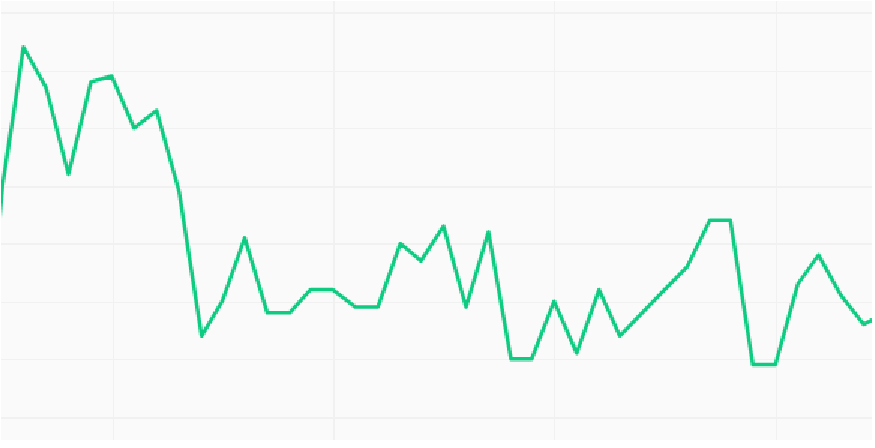
\includegraphics[width=0.45\textwidth]{Figures/linechart.pdf}}}
    \qquad
    \subfloat[\centering Sloupcový graf]{{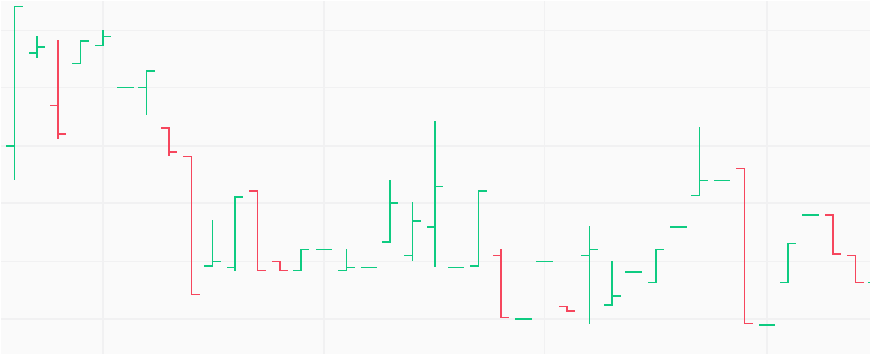
\includegraphics[width=0.45\textwidth]{Figures/barchart.pdf}}}

    \subfloat[\centering Svíčkový graf]{{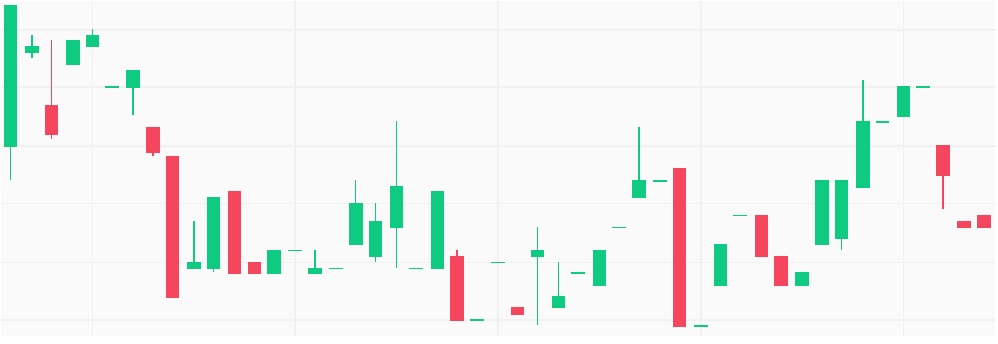
\includegraphics[width=0.45\textwidth]{Figures/candlestickchart.pdf}}\label{subfig:candlestickchart}}
    \qquad
    \subfloat[\centering Svíčka]{{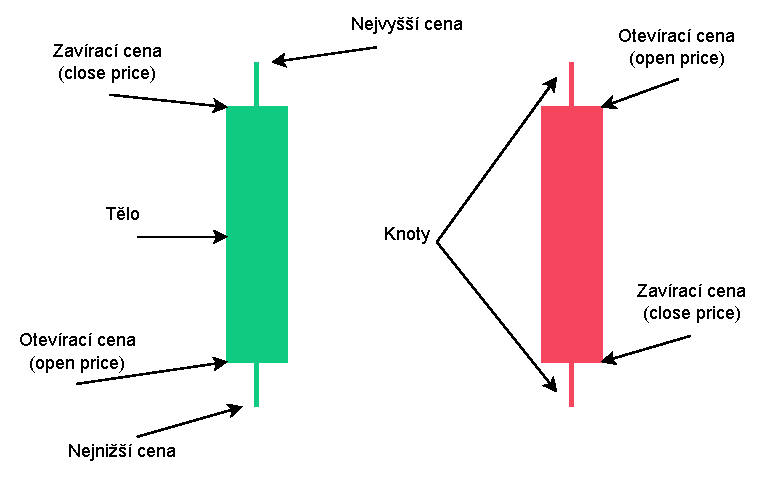
\includegraphics[width=0.45\textwidth]{Figures/candle.pdf}}}

    \caption{Používané grafy a popis svíčky}
    \label{fig:most-used-charts}
\end{figure}


\subsection{Obchodní příkazy}
\label{subsec:market-trade-orders}
Automatizovanou burzu tvoří 2 základní pilíře obchodování. První z nich je obchodní \enquote{kniha} neboli \emph{order book}. Order book není v podstatě nic
jiného než seznam nákupních a prodejních příkazů nějakého aktiva (například kryptoměny). Tento seznam bývá zorganizovaný podle ceny v těchto příkazech.
Druhý pilíř je systém, který se stará o párování těchto prodejních a nákupních příkazů, označovaný jako \emph{matching engine}. Ten spáruje obchodní příkazy
a provede mezi nimi obchod. Ať už jeden obchod, kdy se vypořádávají shodné objemy pro nákup a prodej, nebo více obchodů v případě nerovnoměrného objemu pro nákup a prodej.

Moderní burzy poskytují 2 odlišné typy příkazů. Příkaz typu \textsc{market} jde ihned na order book a otevírá pozici na momentální tržní ceně aktiva. Pokud uživatel
pošle/zadá tento příkaz, je okamžitě vykonán, a to jak v prodejní tak i případné nákupní fázi obchodování. Druhým příkazem, který nabízí možnost automatizace
je \textsc{limit}.
Limit se zadává s hraniční cenou, za kterou je uživatel aktivum ochotný nakoupit nebo prodat. Matching engine se snaží spárovat limit tak, aby byla splněna podmínka
hraniční ceny se spárovaným příkazem. Tato situace je jak pro prodej, tak i pro nákup zachycena na obrázcích \ref{subfig:limit-buy} a \ref{subfig:limit-sell}.

V kombinaci s limit příkazem lze využít další 2 možné příkazy, označované jako \textsc{stop-limit} a \textsc{trailing stop-limit}. Oba přidávají další možnosti,
jak obchodování automatizovat. Stop-limit (\ref{subfig:stop-limit}) příkaz umožňuje přidat další cenový parametr, označovaný jako stop-cena neboli taky aktivační cena.
Tato stop-cena se chová jako zábrana, jelikož nepustí příkaz na order book, dokud není překročena. Například, pokud je aktuální tržní cena aktiva na 100\texteuro, uživatel zadává na burzu stop-limit příkaz k
prodeji se stop-cenou nastavenou na 110\texteuro a limit cenou na 95\texteuro. I přestože je splněna podmínka pro prodej kde je tržní cena vyšší než limitní
a mohlo by dojít k zobchodování matching engine nemůže příkaz zobchodovat, jelikož stop-cena drží příkaz mimo order book. V momentě, kdy tržní cena vyšplhá na
alespoň 110\texteuro, je příkaz puštěn na order book a matching engine může vykonat obchod.
Trailing stop-limit (\ref{subfig:trailing-delta}) posouvá tuto myšlenku ještě o krok dále a umožňuje lepší zachycení trendu tržní ceny.
Tento příkaz počítá procentuální změnu ceny od lokálního
extrému (minimum pro nákup, maximum pro prodej), jakmile rozdíl ceny překročí uživatelem nastavenou hranici, je příkaz zapsán do order booku. Trailing-stop-limit
může mít také nastavenou stop-cenu, tedy musí být splněna podmínka jak stop-ceny tak i procentuálního rozdílu.
Správné nastavení těchto parametrů je důležitým aspektem pro úspěšné zobchodování zadávaného příkazu. Například, pokud při zadávání trailing stop-limit příkazu
je zadaný rozdíl od extrému příliš malý, může být příkaz zobchodován dřív než by to doopravdy bylo výhodné nebo chtěné. Naopak, jestliže by rozdíl byl příliš velký,
nemusí k zobchodování dojít vůbec a příkaz na burze nebude nic dělat.


\begin{figure}[ht]
    \centering
    \subfloat[\centering Oblast pro nákup]{{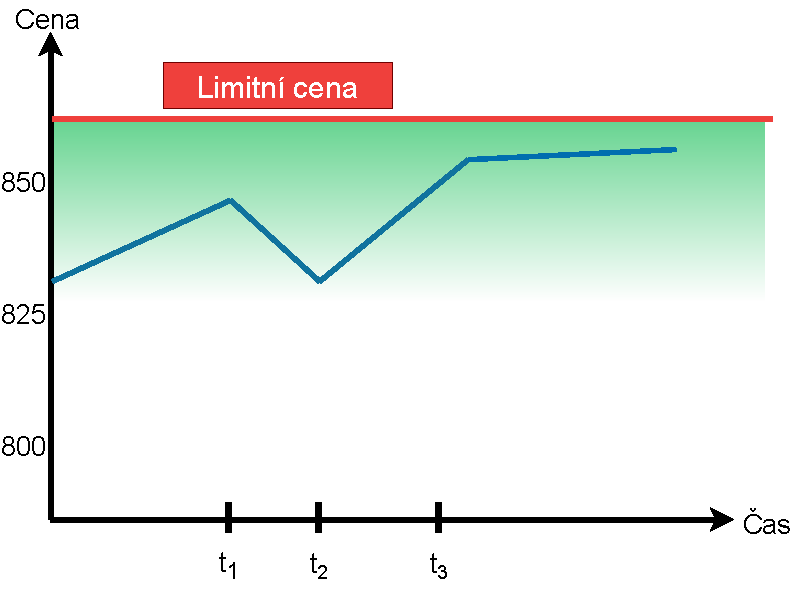
\includegraphics[width=0.45\textwidth]{Figures/limit-chart-buy.pdf}}\label{subfig:limit-buy}}
    \qquad
    \subfloat[\centering Oblast pro prodej]{{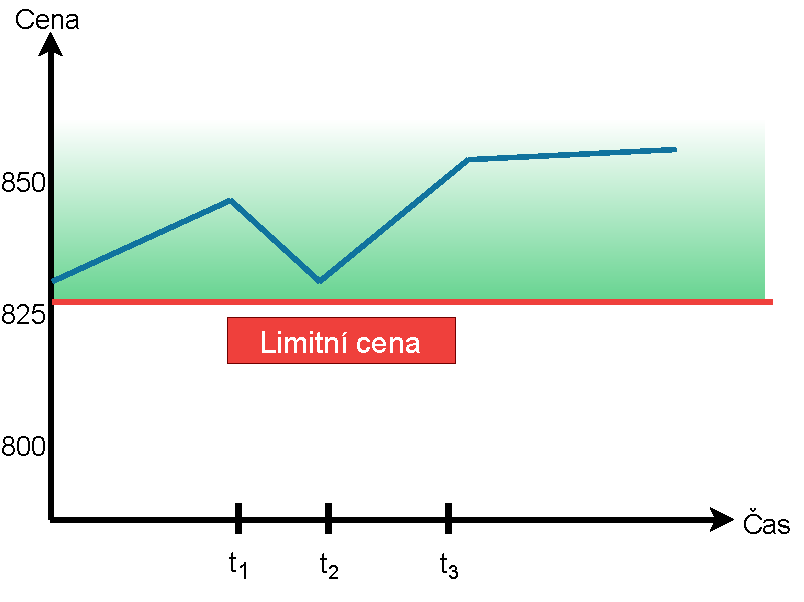
\includegraphics[width=0.45\textwidth]{Figures/limit-chart-sell.pdf}}\label{subfig:limit-sell}}

    \subfloat[\centering \textsc{stop limit} nákup]{{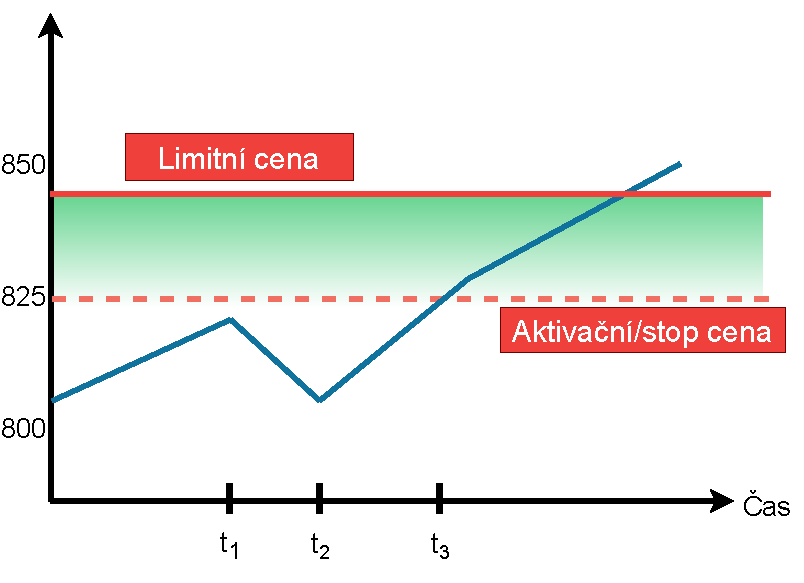
\includegraphics[width=0.45\textwidth]{Figures/stop-limit.pdf}}\label{subfig:stop-limit}}
    \qquad
    \subfloat[\centering Trailing]{{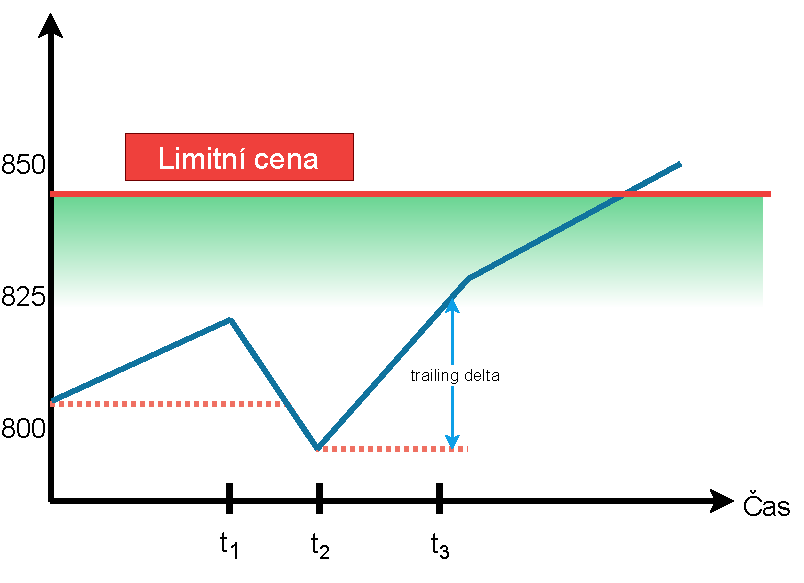
\includegraphics[width=0.45\textwidth]{Figures/trailing-delta.pdf}}\label{subfig:trailing-delta}}
    \caption{Příkaz limit s hraniční cenou}
    \label{fig:limit-orders}
\end{figure}

\subsubsection{Obchodní pozice}
\label{subsubsec:positions}
Burzy umožňují obchodníkům otevírat dva typy pozic: \emph{long} a \emph{short}. Pokud obchodník otevírá long pozici, spekuluje na vzestup tržní ceny aktiva.
Aktiva musí nejdříve nakoupit a následným uzavřením je prodá.
Jestliže obchodník otevírá short pozici (tzv. shortování) spekuluje na pokles tržní ceny. Aktivum tedy nejdříve prodává a následně jej musí nakoupit zpět.
Během shortování obchodník aktivum nikdy nevlastní, ale má je \enquote{vypůjčené} od brokera.


\subsection{Strategie obchodování}
Způsobů, jakým lze obchodovat na burzách může být až nekonečně mnoho. Jelikož se kryptoměnové burzy velice podobají forexovým, mohou se uplatnit podobné
obchodní strategie. Některé strategie mohou fungovat lépe nebo hůře v závislosti na obchodovaném aktivu.
Každý uživatel si může zvolit svou vlastní strategii, tak aby mu vyhovovala, a pár z nich popisuje tato podsekce. \cite{crypto:trading-styles}

\subsubsection{Day trading}
Denní obchodování nebo-li \emph{day trading} se zaměřuje na obchody netrvající déle než jeden den. Tito obchodníci se snaží najít co nejvýhodnější
bod pro nákup a prodej aktiva v rámci jednoho dne a snaží se držet svou pozici nejdelší rozumnou dobu, aby mohli následně svou pozici uzavřít (prodat) se ziskem.
Těchto pozic neotevírají mnoho, spíš jen pár v průběhu obchodního dne.

\subsubsection{Scalping}
\label{subsubsec:scalping}
Tito obchodníci, nazývání \enquote{skalpeři} se snaží vydělat na mnoha malých, ale profitabilních obchodech. Pozice drží otevřené krátkou dobu, většinou pár minut
s nejdelší možnou dobou až pár hodin. Často využívají i \emph{pákového efektu}\footnote{Pákový efekt umožňuje traderovi otevřít pozici s násobenou kupní silou
    a tím i možností jak vyššího zisku, tak i případné ztráty.}. Hlavní podstata této strategie je dosáhnou zisku i z malých změn tržní hodnoty aktiva.
K rozhodování o otevření pozic se opírají o \emph{technickou analýzu}, která bude detailněji popsána v kapitole \ref{chap:TechnicalAnalysis}.

\subsubsection{Swing trading}
Swing tradeři sporadicky otevírají a zavírají pozice na trhu, přičemž své pozice drží i v období několika dnů, nebo týdnů. Čekají na větší cenové
výkyvy (doslova zhoupnutí ceny, odtud název swing trading) a tomu odpovídá i delší doba trvání obchodu. Využívají technickou analýzu ale i fundament
daného aktiva a snaží se odhadnout dlouhodobější trendy.

\subsubsection{Buy-and-hold}
Tato poslední metoda obchodování je čistě dlouhodobá a jedná se pouze o nákupy aktiv. Převážně oblíbená v krypto komunitě dostala tato strategie přezdívku HODL.
Vyhýbáním se prodeje se investoři snaží mířit na výhledový zisk z držení. Podle motivace a filozofie HODLerů je vždy skvělá příležitost nakoupit kryptoměnu a za
žádných okolností neprodávat, ale držet své coiny u sebe.

\endinput